\chapter{Introduction}

  \epigraph{Talk is cheap. Show me the code.}{Linux Torvald}

	\section{Video based tracking}
    The tracking of objects from video recordings is a problem that has gained much popularity in recent years. It is mostly due to its great potential, both in science and for commercial and security applications. Examples include autonomous cars that can drive themselves or the Airbus ATTOL project that allows fully automated take-off, landing, and taxiing based solely on image analysis. A large part of the research effort is focused on creating pedestrian recognition and tracking algorithms to automate the analysis of video surveillance data. Tracking is also widely used in the field of cinema and special effects (VFX), whether to stabilize shots or to realize special effects (e.g., motion capture). In this case, automated tracking on images allows reducing costs and production time. In science, the use of automated tracking, especially in biology and ecology \cite{dell2014automated}, is a rapidly growing field. It avoids the need to invasively mark animals and thus disturbing them. It allows generating a large amount of reliable data, reducing bias, and avoiding a long and laborious manual analysis.

    Object tracking can be separated into two categories: the Single Object Tracking (SOT), where the goal is to detect a single object in a more or less complicated scene, and the Multiple Object Tracking (MOT), where the goal is to detect and track several objects. In this dissertation, we will place ourselves within the MOT framework because it regroups the vast majority of scientific applications. In a scientific experiment, the tracking problem's difficulty is reduced by designing the setup well. In general, the image quality is good, the camera is fixed, and we can optimize the lighting to facilitate object detection. On the other hand, the tolerance to errors is low if one wants to produce reliable data and robust scientific conclusions. A decisive point is the algorithm's performance, which must analyze the data in a reasonable time compared to their production rate and meet the user's material and technical constraints. The ease of installation and use of the software that integrates the algorithm should not be neglected. The users brought to use these software are generally not experts in computer science and image analysis, and the software must be readily installable and usable by all.

    We will first see how tracking is a complex problem and how we can reduce or bypass this complexity. We will then present a non-exhaustive list of existing tracking software applied to scientific fields. Finally, we will see how FastTrack's approach, the software we have created to solve the tracking problem, is different, and in which cases it can be useful.

	\section{The tracking, a not so easy problem}
    The image-based tracking of objects rest on three key steps: the acquisition of the images, which, depending on the acquisition parameters, will condition the difficulty of the tracking and the type of algorithm that can be used, the detection of objects, which consists in separating the objects from the background, and finally the assignment of objects from one image to another allowing to keep track of the objects' identities. Object tracking is generally a complex image processing task \cite{dell2014automated}. Depending on the objects studied, each step can be difficult. For example, animals are highly deformable objects interacting with each other and, making the detection step complex. The scene can be complicated, with objects disappearing behind the decor elements, superimposing each other (the so-called occlusion phenomenon), or entering and leaving the field of view, complicating the detection and the association step.

    Object detection problems can usually be circumvented by the design of the experimental setup whenever it is possible. A fixed point of view and lighting optimization usually allow simple detection by subtracting a background image (without objects) and applying a threshold. For more complicated cases, a wide variety of algorithms are available \cite{yilmaz2006object} and applicable depending on the images' quality. The most common is to detect points of interest in the object. This technique is invariant to the point of view and illumination but requires a good image quality. Segmentation allows to separate the image by area of similarities and thus to detect objects of interest, many algorithms and approaches exist to segment an image. Machine learning can also be applied for objects detection \cite{zhao2019object}.

    Two main classes of algorithms can be distinguished to mitigate association problems. The first class of algorithms uses the object's kinematic quantities, such as direction or position \cite{rodriguez2017toxid, qian2016effective}, to predict or find the position of the object on the next image and thus keep its identity. The error rate of this method remains constant when we increase the number of individuals. It is generally fast, and this makes it a good candidate for real-time tracking applications. The major disadvantage of this approach comes from the error propagation phenomenon. If the algorithm makes an error in the assignment, it has no way to correct the error at the next step, and it propagates to the end of the analysis.
    The second class of algorithms is based on recognizing the object's points of interest, allowing the creation of a "fingerprint" unique to each object. That can be done using either a classical method \cite{perez2014idtracker, bai2018automatic}, or using machine learning \cite{mathis2018deeplabcut, romero2019idtracker}. This technique solves the propagation of errors problem and allows objects to be tracked over time, i.e., across several unpaired videos. For example, an animal can be recognized from one day of experiments to the next, which can be very useful, especially for specific behavioral studies. This method requires an image of sufficient quality to detect markers representative of the object. It also requires more computational resources, thus, an analysis that cannot be done in real-time. However, the main limitation is the number of objects it can track. It is currently limited to about ten objects per image with classical methods before the algorithms' performance degrades significantly. The machine learning approach makes it possible to increase the number of objects at the cost of long computation time and the need to use high-performance machines.

	\section{Existing software}
        Many tracking software already exist. We will make a non-exhaustive list of the most popular ones, separating them into two categories: open-source software and proprietary software.
        \subsection{Proprietary software}
        The proprietary software presented here are closed-source. The user cannot modify the code to adapt the software to his project or check how the tracking is performed. On the other hand, they do not require any computer knowledge and benefit from a support service convenient for users that do not have a lot of computer knowledge. They are an excellent alternative to other options that are sometimes difficult to implement, but their high price can be a hindrance for some users.
        \paragraph{EthoVision XT}
        EthoVision XT is a software developed by the company Noldus. It accompanies the user from the acquisition of images, thanks to a system of experiment templates to the data analysis with a module allowing to visualize standard behavioral parameters. The software is complete and widely used. It is somewhat specialized in the field of behavioral neurosciences. It includes modules for classical behavioral experiments (e.g., water-maze, rats social interaction). It also allows performing live tracking so that users do not have to save images for long experiments.

        EthoVision XT is a mature software. A large number of modules are available as well as a system that allows the user to create its own experiment template. The most significant disadvantage is that the user cannot modify the software or control how the tracking is done. Price can be a barrier for some users, as the software costs a minimum of 5,850 USD without modules, and it is compatible only with Windows.
        \paragraph{Any-maze}
        Any-maze is a software developed by Stoelting Co. It is specialized in the analysis of behavioral neuroscience experiments. It directly integrates tools for standardized tests (e.g., forced swim test, fear conditionning test), allowing fully automatic analysis of these experiments. It can track in real-time or from recorded videos.

        Any-maze is a complete solution for creating and analyzing typical behavioral experiments. It can be purchased with the experimental setup already optimized and calibrated for the software. The Any-maze suite consists of three software packages. The tracking part is available for USD 6,495 or USD 1,500 per year. The software is available for Windows only.

    \subsection{Open-source software}
    Open-source software allows the user to modify and distribute the software. It is the preferred alternative to commercial software. From a scientific perspective, using open-source software increase transparency and lead to easier replicability of scientific results.
    In general, no individual assistance service is provided. The collaborative development of most of these software allows the user to report bugs and participate in the development.
    \paragraph{idTracker}
    idTracker \cite{perez2014idtracker} is a MATLAB library that allows to track multiple objects. It is based on the extraction of a "fingerprint" for each object, and thus a reliable detection without error propagation. The advantage of idTracker is that it can recognize an object over several videos and after a relatively long period of time, which can be useful to track the behavior of individuals over several series of experiments over time. However, IdTracker is limited by the number of objects it can track, currently about twenty, due to the length of the videos necessary for the optimal extraction of the "fingerprint" of each object, which can go up to 30 minutes minimum for a high object density. The required image quality is an important factor and must be at least 150 pixels per animal. The computation time is relatively long, in the order of 0.5 to 2 seconds per image and requires a large amount of RAM. The installation of idTracker can be done without the need to buy MATLAB thanks to the Matlab Run Time Compiler but only under Windows. It is therefore necessary to purchase a MATLAB license for other platforms, and to have a minimal knowledge of the language to set up idTracker.
    \paragraph{ToxTrack}
    ToxTrack \cite{rodriguez2018toxtrac} is a software that implements in a graphical interface the ToxId algorithm \cite{rodriguez2017toxid}. The algorithm extracts objects from the background by applying a threshold. The trajectory pieces between each occlusion are then divided into short and long trajectories based on a user-defined threshold time. A group of long trajectories where all individuals are observed at the same time is then extracted, in this case the assignment is made using the Hungarian algorithm. The short trajectories are then assigned to the corresponding object by correlation between a trajectory identification matrix.
    The authors report that ToxId is as powerful as existing software, very fast, it is possible to track objects in real time. A disadvantage that can be seen in this algorithm is that it only works for a constant number of animals. The initialization of the algorithm requires to have at one moment $t$ all the objects to be tracked simultaneously detectable for a user-defined time $t+dt$. The ui includes tools to define areas of interest as well as statistical analysis of the collected data. We can see that the trajectory correlation matrix does not allow object recognition and that errors with this method are propagative. The software is only available for Windows, the project initially Open-Source shift to a Closed-Source model.
    \paragraph{DeepLabCut}
    DeepLabCut \cite{mathis2018deeplabcut} is a framework that solves the so-called "pose estimation" problem which consists in finding an object and its position, or part of an object, in an image. It can be directly related to the SOT problem if the objects to be tracked are different, for example a right mouse ear and a mouse nose, which can then be found on each image and then associated in the case where there is only one mouse. In the case of several similar objects to be found and associated from one image to another (MOT), this detection will have to be combined with an association to obtain the tracking. Even if DeepLabCut answers a slightly different problem, it can, by its design, be coupled with an external association algorithm to make a tracking software.

    DeepLabCut is directly based on the feature detection algorithm of the DeeperCut framework \cite{insafutdinov2016deepercut}, specialized in the detection of human body movements. The authors of DeepLabCut have studied the performance of this algorithm applied to the field of behavioral neuroscience, such as the detection of a mouse snout, or the paws of a drosophila, and have added tools to easily train the algorithm and test its robustness. It takes advantage of deep learning to solve the "estimation pose" problem. As a reminder, deep learning is a type of machine learning algorithm that consists in training a neural network with several layers. This network consists of several ResNets (residual neural network) that have been pre-trained on the ImageNet database. Deconvolution layers are placed at the output of the ResNets and allow to obtain the probability of presence of the object in the image. The network is then fine-tuned by training it on images where the parts to be detected are annotated. The authors have shown that a performance at least as good as human detection can be obtained with very little training data, of the order of 200 images.

    DeepLabCut, as previously mentioned, is a framework, and despite very good documentation \cite{nath2019using}, it can be difficult to implement for a user with little computer skills. The installation process lasts from 10 to 60 minutes and requires the installation of a GPU and associated drivers to get the most out of the software. In addition, the algorithm requires a lot of computing power and a GPU (NVIDIA GForce 1080 8GB or higher) is strongly recommended. To give an idea, images of 682x540 pixels, analyzed with a last generation GPU, allows to wait for an analysis speed of 30 frames per second, without GPU this time can be multiplied by a factor of 10 where 100 \cite{mathis2018inference}.

    We can see that DeepLabCut is of great interest to find objects in an image with great precision. It is more particularly aimed at behavioral neuroscience where it allows to follow complex movements (e.g. hand finger in a mouse). It will not be suitable for users with little computer knowledge who are interested in larger problems and have a large amount of data to process.
    \paragraph{idTracker.ai}
    IdTracker.ai \cite{romero2019idtracker} is a framework that allows to track animals with almost perfect accuracy. IdTracker.ai takes advantage of deep learning to carry out the tracking. In a first step, each object is segmented by applying a threshold. A convolutional network then classifies each detected blob as containing a single object, or containing several objects. Another convolutional network then finds the identity of each individual throughout the film. To work, this system requires enough data to train the network to recognize each individual. The authors found that a robust tracking can be obtained with only 30 isolated images of each individual as a base, so it is necessary to plan for a minimum of 500 images for a dozen individuals with a minimum of 25 fps. A resolution of 300 pixels per animal is recommended for good tracking accuracy. A limiting factor of idTracker.ai is that it requires a lot of computing time and a lot of RAM, the authors report a duration of about 20 minutes for 8 zebrafish and about 6 hours for 100 zebrafish on about 2000 high definition images. Even if a ui is available to help the user, basic computer and programming knowledge is required, as well as suitable hardware, the use of a GPU is strongly recommended. It is recommended for users who want perfect, fully automated tracking from high quality images and long movies with a powerful machine without time constraints.

    \section{FastTrack: an original approcach}
    We have previously seen the existing software and the different tracking paradigms applied to science. We can see that a fast approach, requiring little computing power, and generalist (can be applied to different systems, variable number of objects, etc...) is missing.
    To fill this void, we designed a software called FastTrack. This software contains two distinct parts:
    \begin{itemize}
        \item An interface where standard image analysis procedures are implemented to detect objects, and a tracking algorithm that allows to keep the identity of objects from one image to another, fast and with a low error rate.
        \item An ergonomic interface allowing the verification and possibly the manual correction of any errors that may have been committed by the tracking algorithm.
    \end{itemize}
    We will notice here the difference in approach between FastTrack and existing software. Instead of developing a system that requires high computing power, which is long but provides fully automated and highly reliable results, FastTrack implements a fast and easy to set up, very generalized method. The correction of the remaining errors is left to the user but can be done natively in the software, the ergonomic interface allowing a fast and efficient correction.
    This solution has several advantages, the first one being that it does not require any programming knowledge, any user can perform a perfect analysis in a very short time. Moreover, it has been shown that the post-processing work can be estimated a priori by an analysis of the geometrical and dynamic parameters of the studied system, which allows the user to know if the software is adapted to his needs. For many of the systems studied, the post-processing is only a quick check. In some cases, if the number of occlusions is too important and a perfect tracking precision is necessary without having to resort to manual correction, another solution must be considered.

    FastTrack is distributed under an free software license and implemented in a modular and fully documented manner. Each user can thus modify the software at his convenience or contribute to it. The tracking algorithm is decoupled from the detection and correction interface which makes it extremely easy to integrate FastTrack into an existing project. The software is easily installed in less than 5 minutes and is compatible with Linux, MacOs and Windows, it can run on modest configurations and Single Board Computer (SBC) such as the Raspberry Pi.


\chapter{Design and implementation}

    \epigraph{Testing can only prove the presence of bugs, not their absence.}{Edsger W. Dijkstra}

	\section{Tools used}
	
	The choice of tools and libraries used in designing a software program is paramount, and several selection factors must be taken into account.
	The first criterion to consider is the license. We chose to put the FastTrack software under a free license (GPL3), which implies that the language used as well as the libraries are also under compatible licenses. The choice of an open-source license is evident in the case of scientific software. The user can then check how the software works, modify it to adapt it to his needs, and share it.
	The second criterion is to choose the libraries used carefully, considering the future of the software so that the user does not have to change libraries if its capabilities prove insufficient as the software evolves. Mature libraries offering long-term support are preferred.

	In this perspective, FastTrack has been implemented in C++ using the Qt \cite{Qt} and OpenCV \cite{opencv_library} libraries for the graphical interface and image analysis, respectively. Unit tests are performed using the Google Test library.

	C++ is a computer language created by Bjarne Stroustrup in 1985. Offering high performance, it is standardized by the International Organization for Standardization (ISO). It is the language of choice for image analysis applications and the creation of complex graphical user interfaces.

	Qt is an open-source GUI library created by Haavard Nord and Eirik Chambe-Eng, both physicists, in 1991 when developing ultrasonic image analysis software. With extensive documentation and a large community, it is very mature. It allows creating graphical user interfaces for Linux, Mac, and Windows with the same source code.

	OpenCV is an open-source image analysis library created by Intel in 1999. Very complete and efficient, it has become the reference in image analysis for both research and commercial applications.

	Google test is a suite for automating unit tests in C++. OpenCV notably uses it. The purpose of unit tests is to verify that each part of the program works as expected. This practice has several advantages: detecting more easily possible errors during the implementation of new features and facilitating the development of the software when it grows in size to avoid any error inclusions. This series of tests are automatically performed on each new commit, see section~\ref{}.

	\section{Implementation}
	FastTrack's operation can be divided into three parts: the detection of objects, the association of objects from one image to another, and finally, a correction step.

	Each analysis begins with the opening of a sequence of images or a video file. The user can choose between two types of interfaces, an interactive interface where he can only open one film at a time. It allows the user to see, in real-time, the impact of parameters on the images. Which facilitates the determination of the optimal analysis parameters. A second interface allows many movies to be opened simultaneously, either by giving a parameter file or selecting the parameters in the interface. It is useful when the user wants to analyze many movies for which he already knows the optimal analysis parameters.

	Both interfaces can be used in a complementary way. The user can find the optimal parameters with the interactive interface and then automate the analysis of many movies by adding them in batches in the software.


	\begin{figure}[h!]
    \centering
    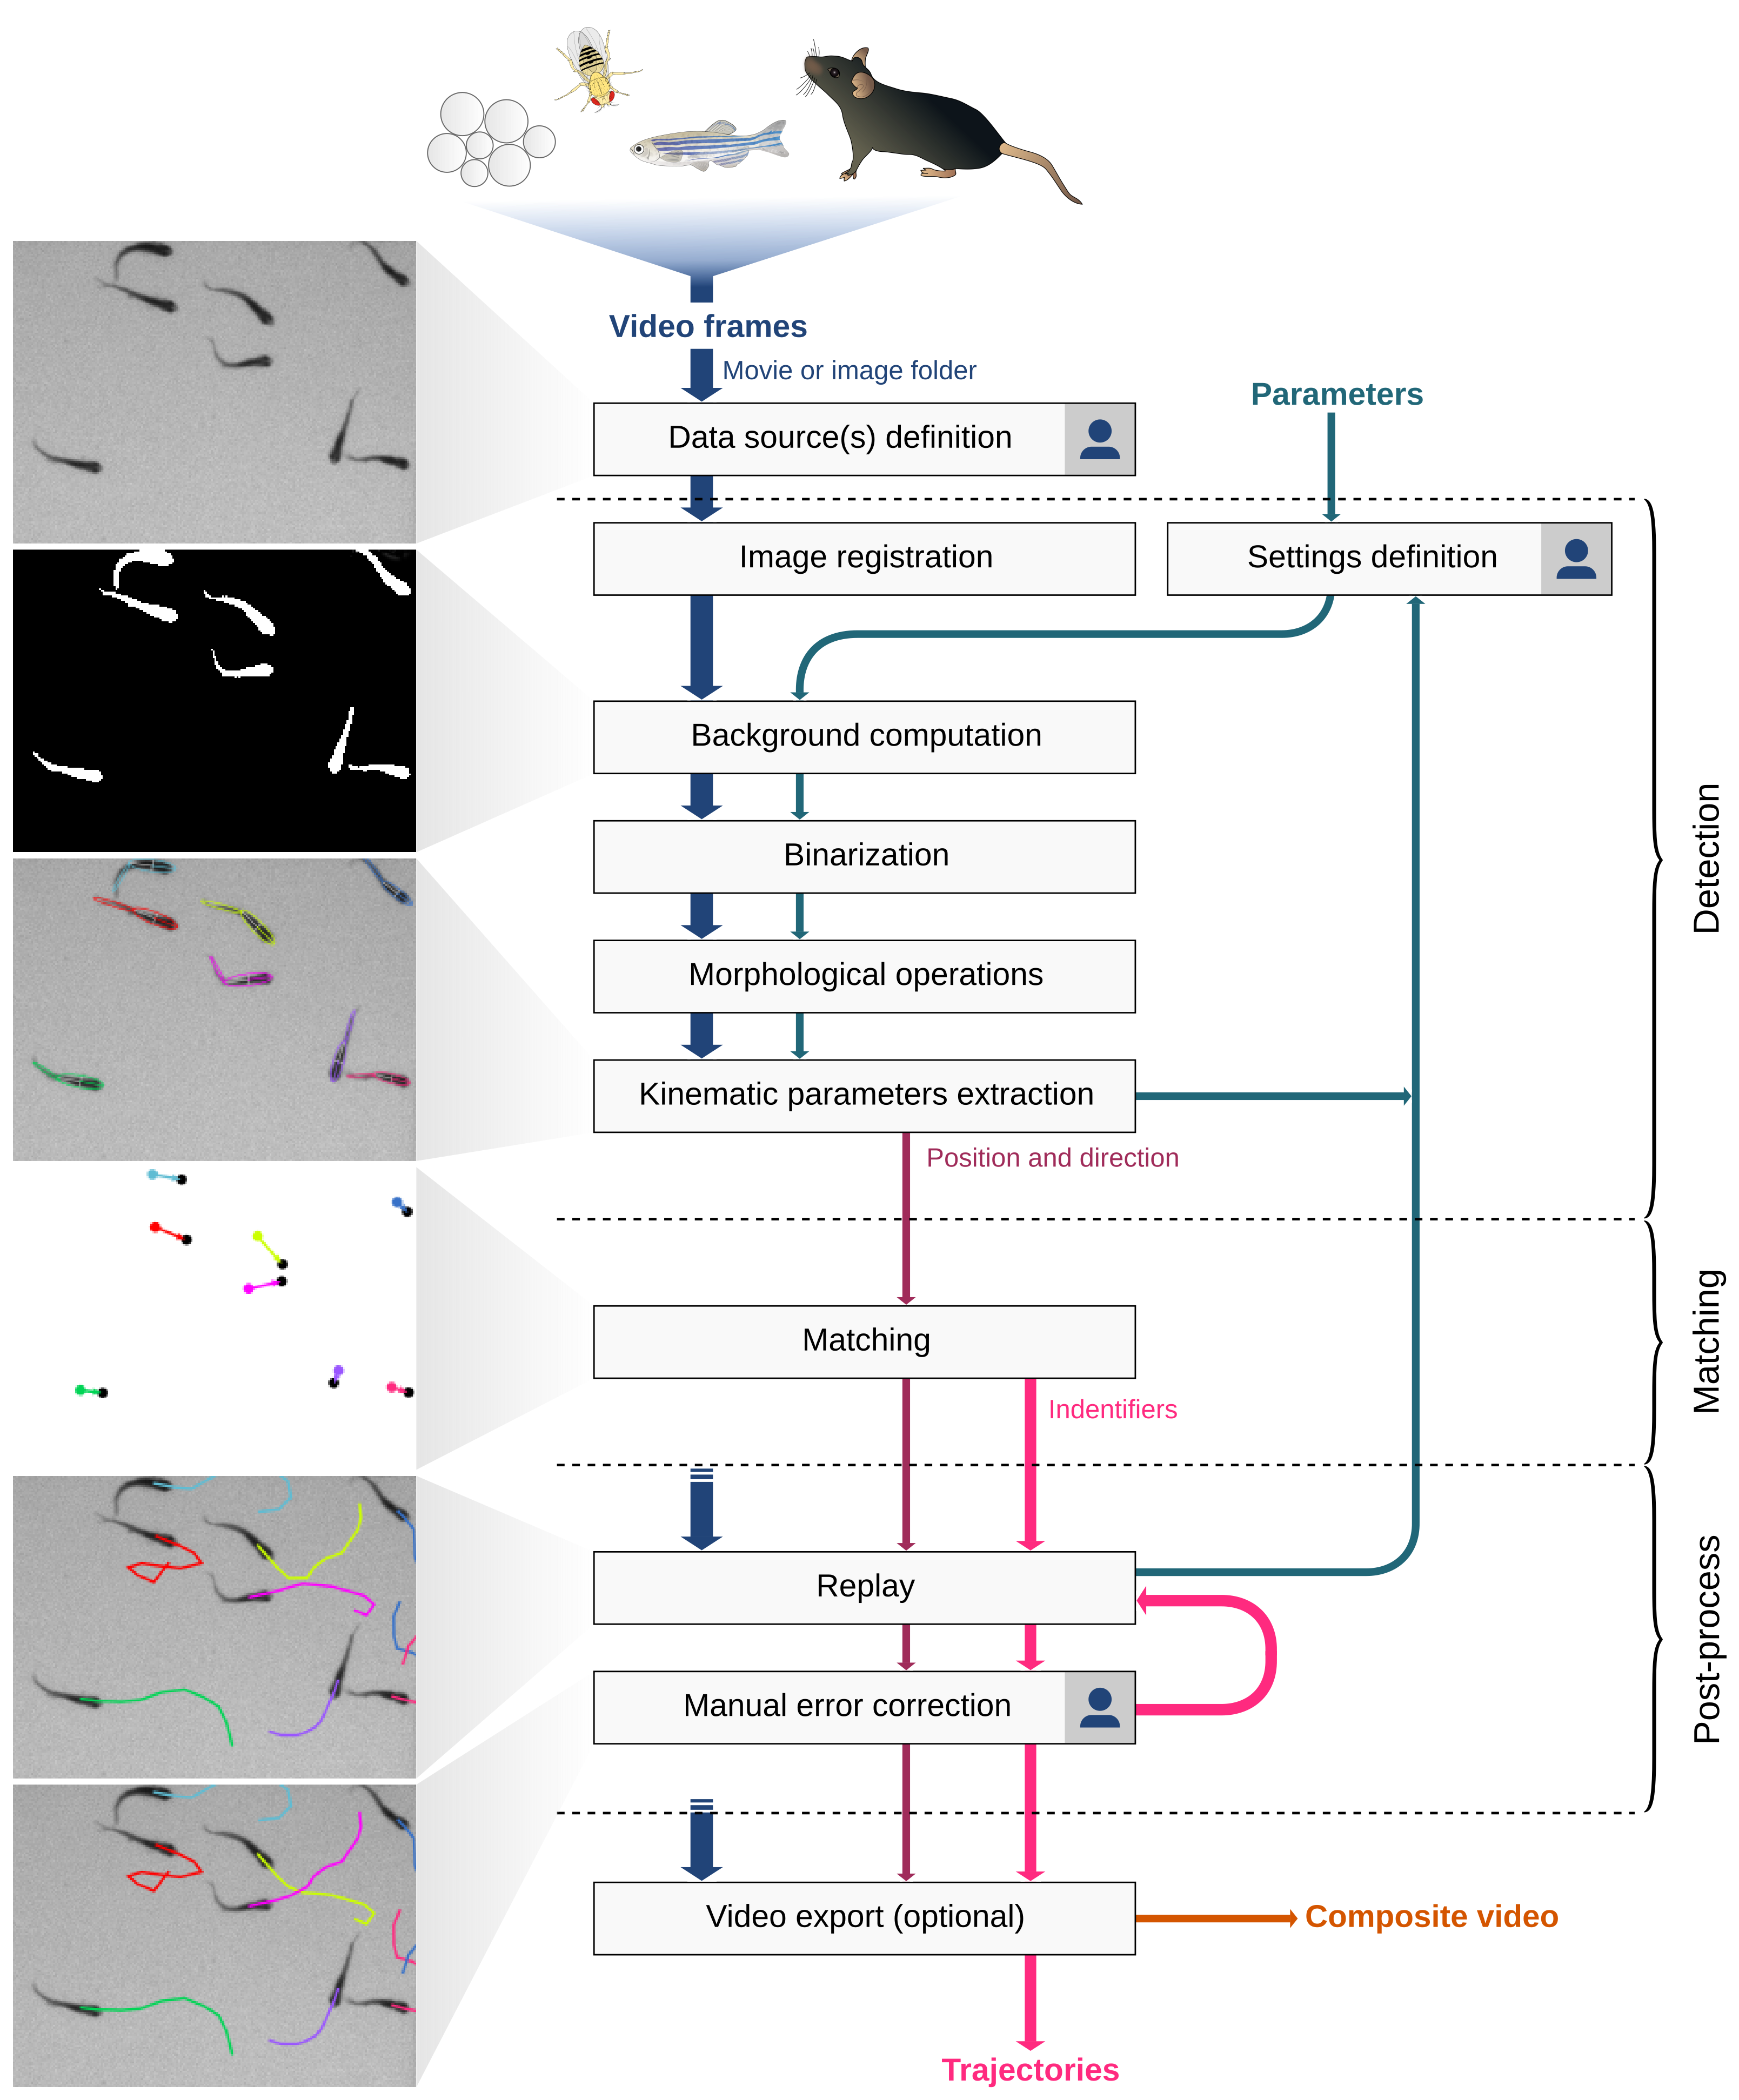
\includegraphics[width=0.75\textwidth]{part_1/assets/Figure_1.png}    
    \caption{\textbf{FastTrack flux de traitement.} Il se divise en trois parties distinctes : la détection, l'association et le post-traitement.}
    \label{part_1:fig_1}
    \end{figure}
	
	
		\subsection{Detection}
		The purpose of the detection step is to extract each object's kinematic parameters, which will then be used in the association step. FastTrack includes a collection of image analysis filters that allow the user to optimize object detection without external software.
		\paragraph{Background Calculation}
		Each analysis starts by calculating a background image. If the user already has a previously saved background image, he can open it directly in the software. Otherwise, three calculation methods are possible:
		\begin{itemize}
			\item Projection of maximum intensity.
			\item Projection of minimum intensity.
			\item Projection of the average intensity.
		\end{itemize}
		All three methods are based on the same principle. The user chooses $n$ images in the sequence. The software will project in the direction perpendicular to the image (along the time component) either the maximum, minimum or average of the sequence. In practice, the maximum (resp. minimum) will be projected if the objects are darker (resp. lighter) than the background so that the objects disappear and thus obtain the background. The user can make the registration of each image before the projection in order to correct a possible camera movement.
		
		\paragraph{Registration}
		The user can choose to register the images. Three methods are proposed in the software. Each method is implemented in a pyramidal way, i.e., the registration is first carried out on a degraded image to roughly correct the displacement. The correction is then refined by increasing the image quality until the original quality is reached. This speeds up the process, as registration is often a relatively time-consuming process.


		The first method proposed is phase correlation. It allows correcting the translational movements between two images using the Fourier theorem in the frequency domain. This method is swift but remains limited to small translational movements only.


		The second proposed method is the Enhanced Correlation Coefficient (ECC) method. In FastTrack, it is restricted to correcting translational and rotational movements only. It consists of using the correlation coefficient as a measure to find the best transformation between two images. This method's advantage is that it is relatively fast, since the non-linear optimization problem can be solved in a linear way. It is efficient for noisy images and having photometric distortions (contrast, brightness).


		The third method is a method based on the identification of key points. It allows for correcting movements and deformations (homography). The key points (about 500) are automatically determined on two images thanks to the ORB algorithm \cite{}. These points are then associated two by two using the RANSAC algorithm \cite{} to find the best transformation between the two images. This method, more precise, requires a sufficient image quality to be able to discern key points.
		
	\begin{figure}[h!]
    \centering
    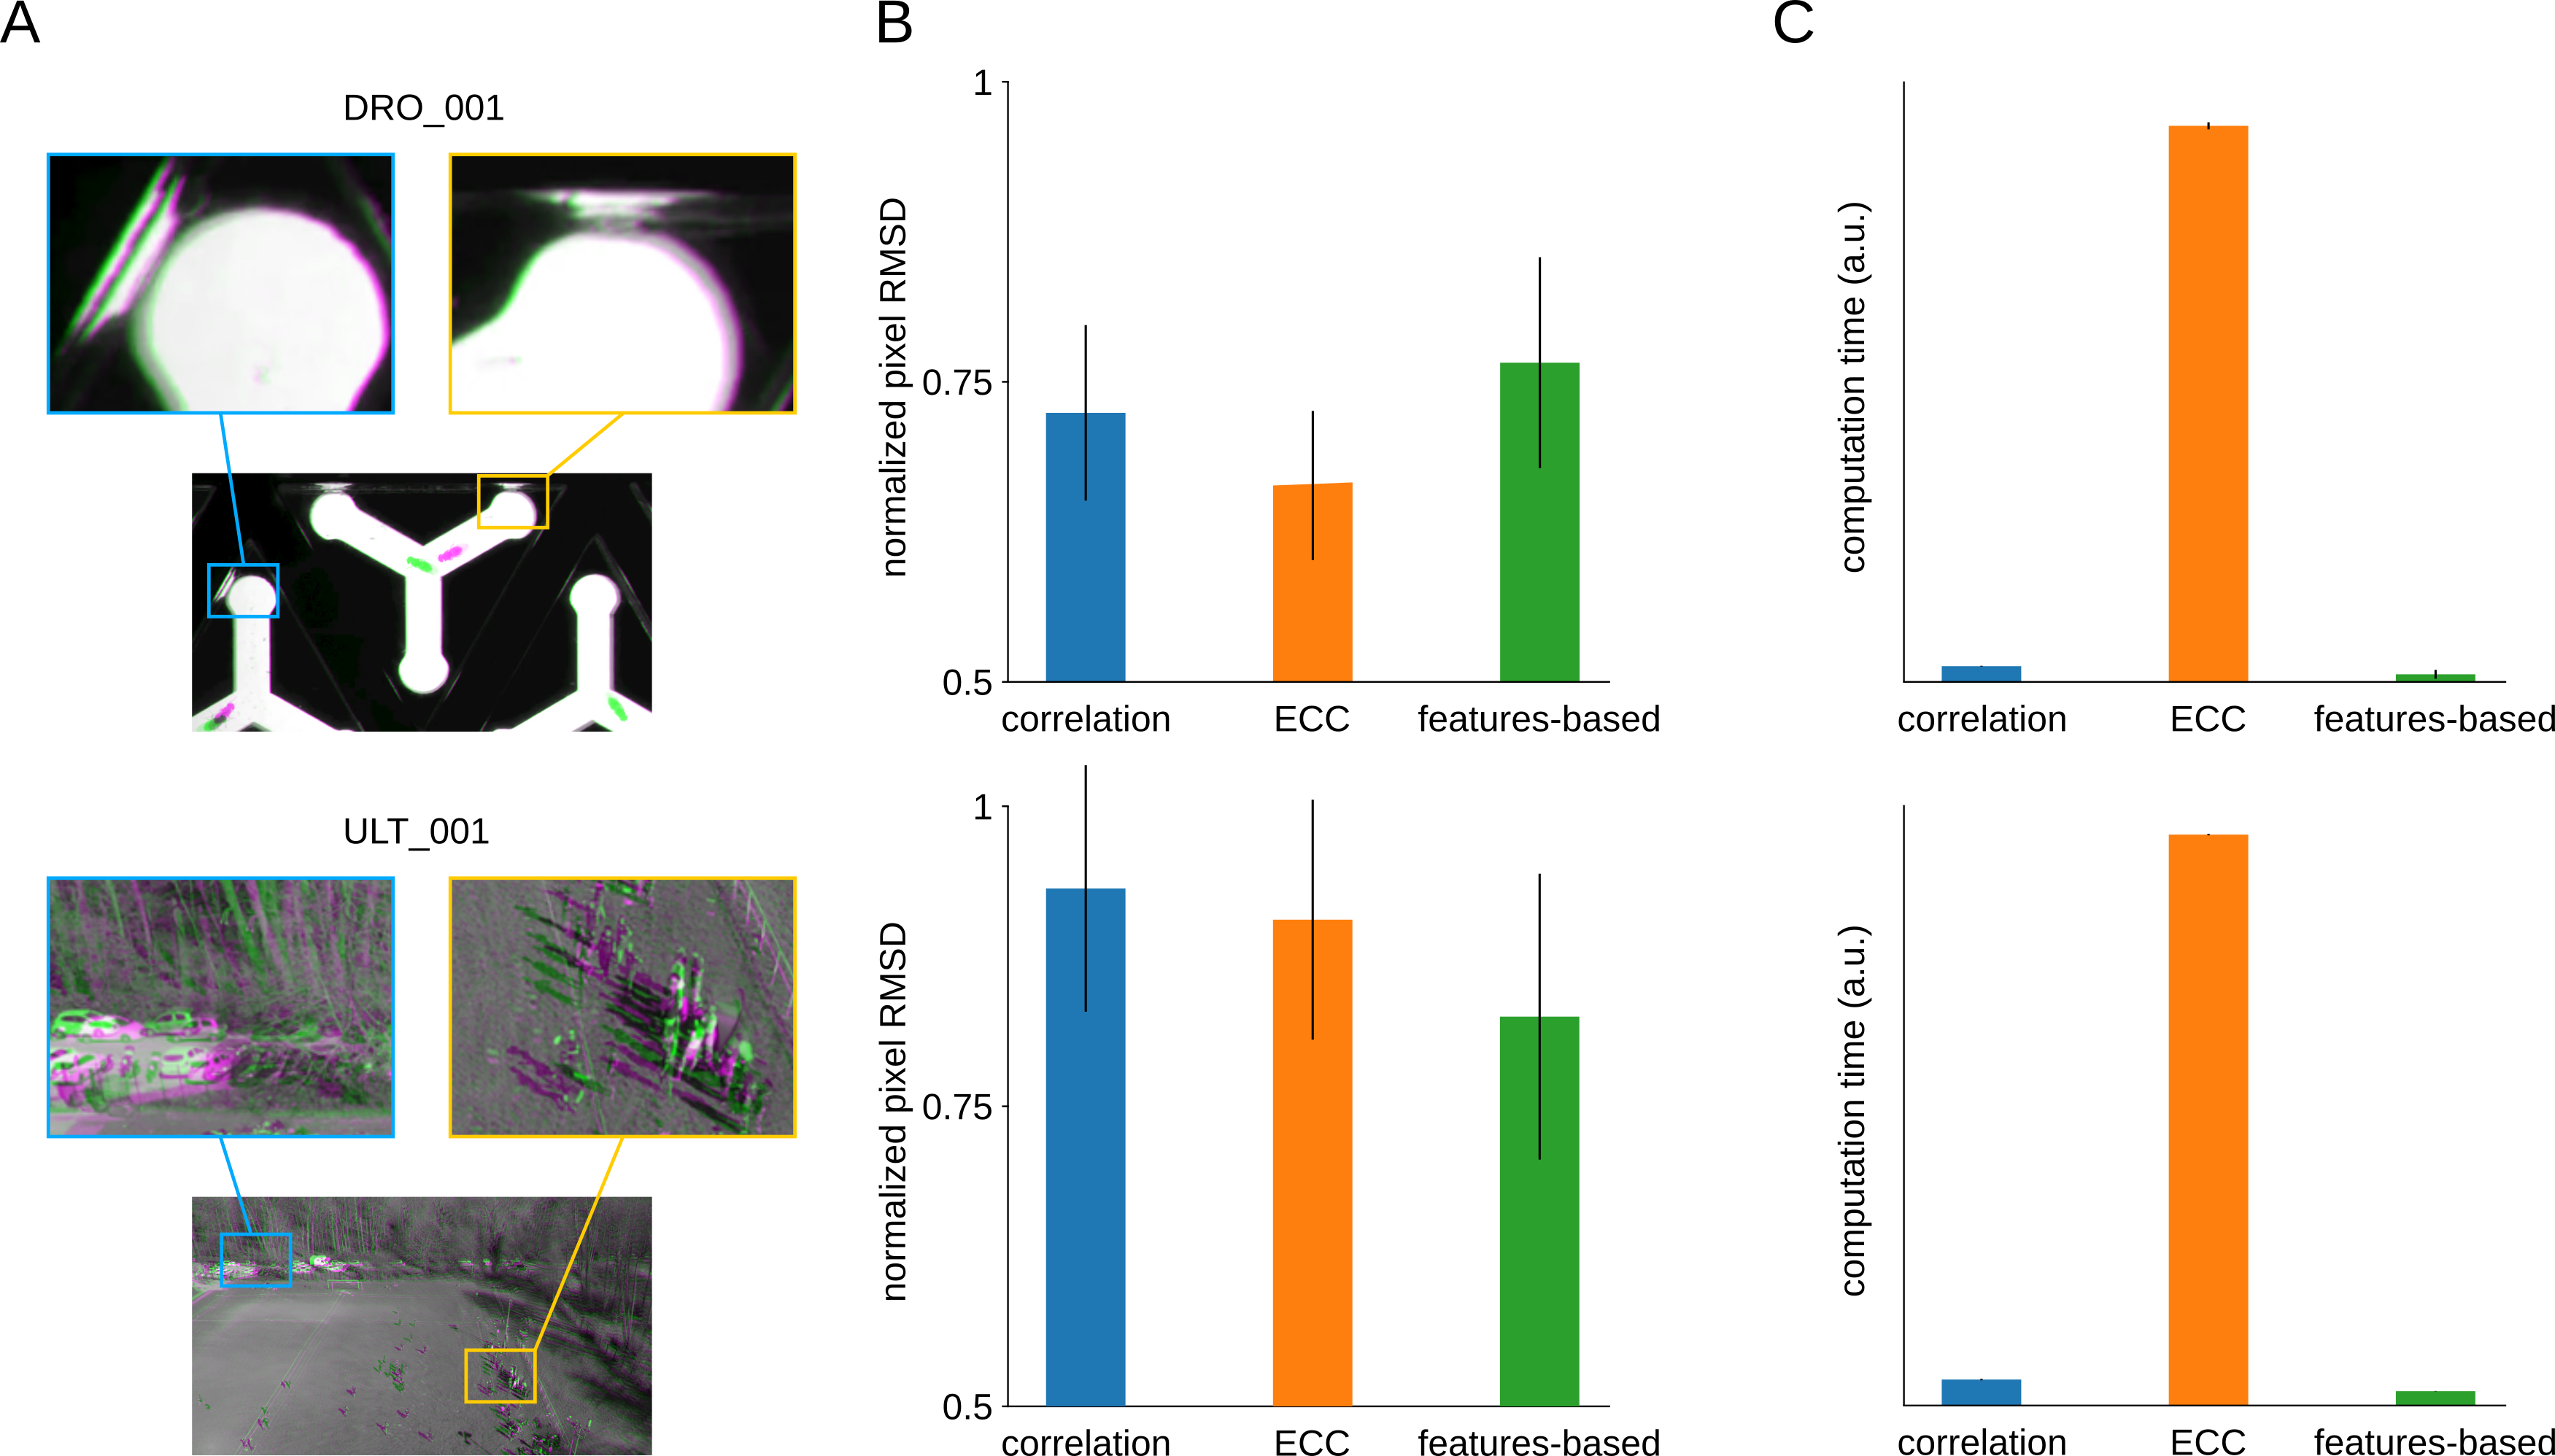
\includegraphics[width=1\textwidth]{part_1/assets/Figure_2.png}    
    \caption{\textbf{Registrations.} Deux films avec une dérive sévère sont utilisés comme référence (DRO\_001 en hautn ULT\_001 en bas). (\textbf{A}) Comparaison entre une image (magenta) avec la première image (vert), avec agrandissement des détails en insert. (\textbf{B}) Déviation moyenne carrée (RMSD) de l'intensité des pixels avant et après registration, moyennée sur toutes les images et normalisée par la RMSD sans registration pour les trois méthodes. Barres d'erreur : déviation standard. (\textbf{C}) Temps moyen relatif pour les trois méthodes (unités arbitraires). Barres d'erreur : déviation standard.}
    \label{part_1:fig_2}
    \end{figure}
		
		\paragraph{Binarization}
		Each image is then binarized by subtracting the background image from it and defining a threshold value. In the interactive mode, the user can see the impact of the parameters on the image, which makes it easier to adjust the binarization threshold. The software also detects if the background is darker (resp. lighter) than the objects allowing to have at the end of this operation a binary image where the pixels belonging to the object are equal to 1, and the pixels belonging to the background are equal to 0.
		\paragraph{Morphological operation}
		A set of morphological operations (dilation, erosion, opening, etc...) can be performed on the binary image to improve detection and eliminate possible artifacts. Different shapes and sizes of cores are available.
		\paragraph{ROI}
		The user can select a region of interest and exclude the rest of the image from the analysis. This speeds up the analysis process and avoids the detection of interfering objects. In interactive mode, this ROI can be drawn directly on the image.
		\paragraph{Sort}
		To exclude objects that are too small for noise or too large, for example, two objects on top of each other, the user must select two characteristic sizes. The objects are colored either red or green in interactive mode depending on whether their size belongs to the selected size range.
		\paragraph{Extracting Kinematic Parameters}
		Based on the binary images, the software will detect the contour of each object. An essential step in any tracking procedure is the extraction of the parameters that will be used in the association step. It is generally in the choice of its quantities that the tracking algorithms differ to specialize to a given type of object. In FastTrack, the parameters extracted are the center of mass, the orientation, the area, and the object's perimeter. Its quantities are quickly calculated and general enough to adapt to a wide variety of objects.

		To do this, FastTrack calculates the object's equivalent ellipse from the second-order moments of the binary image. This procedure is accelerated by directly using the contour thanks to Green's formula \cite{}. The orientation of the object is given by the major axis of the equivalent ellipse. Its direction is determined by projecting each pixel of the object on the major axis of the ellipse. The skewness of the distribution of distances of the projected points from the center of mass is then calculated. The skewness sign is a robust indicator of the asymmetry of the object with respect to its major axis from which the direction of the object can be determined.

		For deformable objects, the previously calculated direction may be different from the direction of movement. For example, in the case of zebrafish, it deforms its body periodically to move. Only the head is directed in the same direction as the movement. This is why the object is decomposed into two equivalent ellipses. The user can then choose which ellipse best represents the direction of movement.

		\subsection{Association}
		The purpose of the association step is to keep the objects' identity from one image to another. To do so, FastTrack uses a method derived from \cite{}, which takes advantage of the fact that each object's position, area, perimeter, and direction changes very little from one image to another.
		For each pair of objects (i,j) belonging to two successive images, two costs are calculated.
		We defined the hard cost as follows:
        $$
        \left\{
        	\begin{array}{ll}
        		h_{i,j} = 1 & \mbox{if } r_{i,j} < h_{d} \\
        		h_{i,j} = \inf & \mbox{else }
        	\end{array}
        \right.
        $$
        With $r_{i,j}$ the distance between objects i and j, $h_{d}$ a threshold representing the maximum travel distance allowed between two successive images. The hard cost allows discarding obvious impossible assignments to speed-up the computation. It is essential with a non-constant number of objects because it allows new objects entering the field of view to be assigned with new identities.
		The soft cost is defined as follows:
		$$
        c_{i,j} = \frac{r_{i,j}}{s_d} + \frac{\delta\alpha_{i,j}}{s_{\alpha}} + \frac{a_{i,j}}{s_a} + \frac{p_{i,j}}{s_p}
		$$
		where $\delta\alpha_{i,j}$ is the angular difference, $\delta a_{i,j}$ the area difference and $\delta p_{i,j}$ perimeter difference between objects i and j. To compare these quantities expressed in different dimensions and magnitudes, we need to normalize them. We define the soft normalization coefficients: $s_{d}$, $s_{a}$, $s_{p}$ and $s_{\alpha}$. These coefficients represent the typical value of the parameter that they normalize.
        We can construct the cost matrix:
		$$
        C_{i,j} = \left\{
        	\begin{array}{ll}
        		c_{i,j} & \mbox{si } r_{i,j} < h_{d} \\
        		\inf & \mbox{sinon }
        	\end{array}
        \right.
        $$
        This cost matrix is, in general, rectangular because the number of objects can vary from one image to the following. A memory parameter can be selected to assign a new identity to an object that disappears on more than the selected number of images. In this case, we remove the row corresponding to this object from the cost matrix.
        We want then to find the best possible association. This problem is called the rectangular assignment problem and can be solved exactly by using the Hungarian algorithm. FastTrack uses the Kuhn-Munkres implementation in C++ to solve this problem.

        \subsection{Automatic tracking parameters}
        Finding the optimal tracking parameters is necessary to have a tracking accuracy as good as possible. FastTrack can automatically determine a neutral set of soft normalization factors $s_r$, $s_\alpha$, $s_A$, and $s_p$ to help the user. These factors allow comparing terms of very different nature and amplitude into a single cost function. The set of parameters automatically found by FastTrack will give each term the same weight inside the cost function. Therefore, the user must perform parameters' fine-tuning, with some system insight, to get the best set of parameters possible.

        It is intuitive to use the standard deviation of the increments of each kinematic parameter. However, some trajectories are needed to estimate the standard deviations. We set up an iterative, rapidly-converging algorithm to perform this talk.

        Let us use $ZFJ\_001$, a slightly oversampled movie, with many occlusions and objects of different sizes to illustrate the algorithm's details. For simplicity, let us use only the position, angle, and area as kinematic parameters. There is no gain to expect by adding the perimeter parameter because objects' shapes are very similar. The Figure~\ref{part_1:fig_5}-A. shows a snapshot of this movie.

        In order to evaluate the distributions of $dr$, $d\alpha$ and $dA$, we start by tracking the movie setting the hard parameters and random soft parameters. The resulting distributions are shown in Figure~\ref{part_1:fig_5}-C to E. For kinematic parameters whose differential values can be positive or negative the distribution is fitted by a Gaussian function and the soft parameter is set to the standard deviation. For instance with the angular difference $d\alpha$ the fit reads:

        \begin{equation}
        f(d\alpha) = \frac{1}{s_\alpha\sqrt{2 \pi}} \; e^{-\frac{d\alpha^2}{2 s_\alpha^2}}
        \label{eq:fit_Gaussian}
        \end{equation}

        and $s_\alpha$ (orange bar in Figure~\ref{part_1:fig_5}-D) is stored as the soft parameter to use during the next iteration.
        The computation of the soft parameter for displacement of $s_r$ is different since distances can only be positive. Assuming that the displacements along the $x$ and $y$ axes follow two independent Gaussian processes, the resulting displacement follows a $\chi$ distribution with $2$ degrees of freedom, and the fit reads (see Annexe~\ref{part_1:fig_5} for de detailed derivation):

        \begin{equation}
    f(x)
        \label{eq:fit_chi}
        \end{equation}

        where $s_r$ (orange bar in Fig~\ref{part_1:fig_5}-C) is stored as the soft parameter to use for the next iteration.

        Once all soft tracking parameters have been derived from the distributions, the software recomputes new trajectories with these updated parameters. This iterative process, depicted in Figure~\ref{part_1:fig_5}-B, is run until the tracking parameters converge. In practice, the convergence is very fast, regardless of the initial position in the parameters space. We drew $100$ sets of seed parameters from uniform distributions spanning large intervals, and convergence has been attained in very few iterations for all parameters Figure~\ref{part_1:fig_5}-F.

        FastTrack's implements this algorithm by taking the kinematic quantities' sample standard deviation to increase speed and efficiency. The convergence criterion implemented is that soft parameters should vary less than $10^{-3}$.

        To characterized the resulting tracking, we computed the amount of swaps with respect to the ground-truth:

        \begin{equation}
        P_{swap} = \frac{N_{swap}}{N_{obj} - n_{ap}}
        \label{eq:Pswap}
        \end{equation}

        with $N_{swap}$ being the total number of swaps, $N_{obj}$ the total number of objects on all frames and $n_{ap}$ the number of times a new object appears. If the number of objects is constant and noted $n$, then $n_{ap} = n$ and $N_{obj} = nT$, with $T$ the number of frames in the recording, such that $P_{swap}$ can be simpliefied:

        \begin{equation}
        P_{swap} = \frac{N_{swap}}{n(T-1)}
        \label{eq:Pswap_constant}
        \end{equation}

        $P_{swap}$ converges very fast to a value that is nearly-optimal. For $77\%$ of the parameter sets $P_{swap}$ is decreased or remain equal, with an average drop of $0.0119$ ($155$\% of the converged value), while for 23\% of the parameter sets $P_{swap}$ is increased with an average rise of $0.0011$ ($14$\% of the converged value). Thus, the expected difference is $-0.0090$ ($116$\% of the converged value) for this movie. Therefore, the automatic parameters are an excellent starting point in the general case. The user can fine-tune the weights given to the kinetic parameters to consider the specificities of each movie.

        We computed the converged soft parameters $\hat{s}_r$, $\hat{s}_\alpha$ and $\hat{s}_A$ for several sampling rates of $\tau>1$ (Fig~\ref{part_1:fig_5}-H to J). We used these parameters to track the $ZFJ\_001$ movie at different $\tau$ and compute $P_{swap}$. A comparison between $P_{swap}$ and $P_{inc}$ as a function of $\tau$ is shown in Fig~\ref{part_1:fig_5}-K. This comparison illustrates that $P_{swap}$ is a noisier measurement of a movie's trackability than $P_{inc}$ and confirms that the iterative algorithm produces trajectories with a number of errors that is close to the statistical limit.

        \begin{figure}[h!]
        \centering
        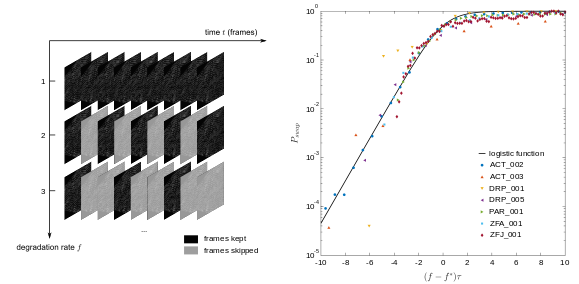
\includegraphics[width=1\textwidth]{part_1/assets/Figure_5.png}
        \caption{\textbf{}}
        \label{part_1:fig_5}
        \end{figure}


		\subsection{Manual correction}
        FastTrack integrates a manual tracking correction tool. Once the analysis is completed, the result can be displayed in an ergonomic interface created solely for this purpose. The user can replay the film by superimposing the results of the analysis on the original movie. The user can interactively see each object's parameters. More importantly, the user can also directly correct tracking errors by deleting objects or exchanging objects' identity.
        This interface is designed with ergonomics and performance in mind. Keyboard shortcuts and an on-the-fly selection of objects by clicking on the video allow the user to check and correct the analyses quickly. It is also possible to record a film with the tracking results overlay superimposed.
        This manual correction interface makes it possible to shift the workload from the traditional pre-processing of data to the tracking result's post-processing. In general, tracking software will reduce user inputs and improve tracking by using the raw images' pre-processing and the conception of system-specific tracking algorithms. With FastTrack, the pre-processing step is reduced to the minimum to remain general and be applied to a wide variety of systems. To compensate for this, FastTrack provides a correction tool. We will see in the following chapter that this method can save the user much time because the correction time is in genral lower than the conception and computational time of system-specific tracking algorithms.

		\subsection{Analysis}
        A question that comes back a lot from users' feedbacks is what to do after the tracking. FastTrack only takes care of the tracking, and statistical data analysis is not implemented in the software. After the tracking, the software generates several files containing the results and the tracking parameters. The result file is named tracking.txt, and it contains the raw data of the analysis with one image and one object per line. This format is compatible with the most used analysis software (R, Python, Julia, spreadsheet). Examples in Python and Julia are available in the documentation to get started.

	\section{Deployment}
		\subsection{CI/CD}

        \begin{figure}[h!]
        \centering
        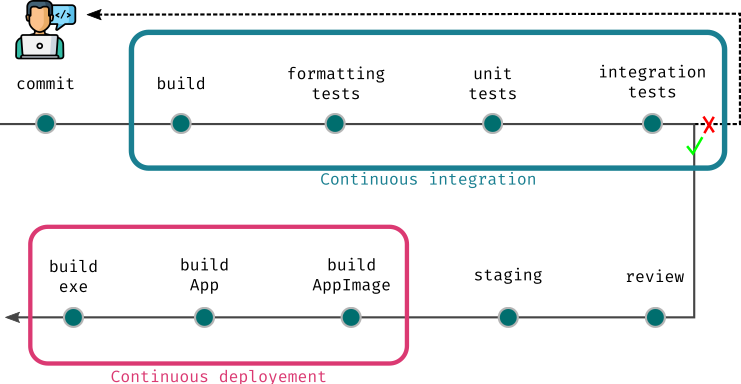
\includegraphics[width=1\textwidth]{part_1/assets/Figure_cicd.png}
        \caption{\textbf{FastTrack CI/CD workflow.}}
        \label{part_1:fig_cicd}
        \end{figure}

        The deployment is one part that should not be overlooked in software design, and two aspects are crucial to consider. From the user's point of view, the software must be easy to install on supported platforms and with fewer bugs as possible. From the maintainer's perspective, the deployment part must be easily achievable and reproducible so that patches and new functionalities can be quickly integrated. From the developer's perspective, the source code's consistency and correctness have to be tested at each change to avoid introducing bugs and facilitate collaboration between developers.  With this in mind, FastTrack follows the CI/CD philosophy \cite{shahin2017continuous}\cite{wikstrom2019benefits} taking advantage of the new GitHub Actions system.

        Continuous Integration (CI) is a set of practices designed to integrate changes into the project in an automated manner quickly. It is coupled with the automation of unit testing. FastTrack takes advantage of GitHub's CI/CD system called Actions. With each new (commit\footnote{Action to send the list of changes made in the version management system}) or new (pull-request \footnote{Action to request the addition of changes to the project}), a series of tests is automatically triggered. These tests will check the proper functioning of the tracking algorithm and the formatting of the source code. Only the changes that pass the tests can be integrated into the project, which guarantees the reproducibility of the analyses and the consistency of the source code and documentation.

        Continuous Delivery (CD) automates the delivery of the software in its final form. It allows changes to be quickly integrated into the software without manually doing it for each supported platform. In the case of FastTrack, the CD is implemented using GitHub Actions, and a new version of the software is compiled for Linux, MacOs and Windows with each new commit that is integrated into the main branch. Stable versions of the software are compiled at regular intervals of the development. This system is a significant time-saver for multi-platforms software like FastTrack. It allows the user to always have the latest patches and features available, the developers to collaborate easily on the project, and the maintainer to quickly produce binaries for the supported platforms.

        FastTrack natively supports the three most commonly used platforms: Linux systems with an AppImage that supports all distributions, Windows with an installer, MacOS with an App. The latest stable version can be downloaded from the website \url{http://www.fasttrack.sh}, thenightly build version from \url{https://github.com/bgallois/FastTrack/releases}. The procedure to compile the software itself is available in the developer's documentation.

		\subsection{Documentation}
        FastTrack offers extensive documentation that covers the installation and utilization of the software. Developer documentation with a documented API and a compilation guide is also available for users wanting to integrate FastTrack in their software or workflow.
        \paragraph{User} User documentation is available at \url{https://www.fasttrack.sh/UserManual/docs/intro.html}. This documentation is generated from the project, and users can contribute to it at https://github.com/bgallois/FastTrack/. It contains all the information needed to use the software, as well as instructional videos to help the user get started with the software.
        \paragraph{Developer} Developer documentation is available at \url{https://www.fasttrack.sh/API/index.html}. It is automatically generated by the Doxygen software from the documentation in the FastTrack source code. It contains all the information necessary for developers who want to modify or contribute to FastTrack.

\chapter{Movies dataset}
    To demonstrate that FastTrack can analyze movies from various systems, we have compiled a database of movies named $TD^2$. This database can be downloaded at \url{https://data.ljp.upmc.fr/datasets/TD2/}. The films either come from data already published in the literature or provided to us by the authors themselves. All the movies are under a CC-BY-NC-SA license. Each movie is identified by a 3-letter code defining the system (e.g., ACT: active matter, ZFA: zebrafish adult...) and three digits to index films from an identical system. $TD^2$ currently regroups 41 films, including different types of objects of very different nature and size
    \begin{itemize}
    \item 7 species of animals from fish to flies,
    \item cells,
    \item active particles,
    \item microfluidic drops,
    \item macroscopic objects such as ultimate players or cars.
    \end{itemize}
    A video giving a quick overview of all the systems used is available at \url{http://www.fasttrack.sh/images/illustrations/mockups/trackingExample.webm}.

    Another essential aspect to consider is the number of objects per film and their possible appearances, disappearances, and overlaps. In 22 films out of 41, the number of objects is variable, and objects come and go out of the camera field during recording. In 19 films out of 41, objects may overlap, creating an occlusion phenomenon that the software has to manage to preserve the identity of the objects.

	\begin{figure}[h!]
    \centering
    \includegraphics[width=1\textwidth]{part_1/assets/Figure_td2.png}    
    \caption{\textbf{$TD^2$.}}
    \label{part_1:fig_5}
    \end{figure}


\chapter{Results}

    \section{Performance}
    To assess FastTrack's performance, we ran a benchmark comparing FastTrack, Idtracker.ai, and ToxTrac. These software have substantial intrinsic limitations compared to FastTrack. Both require an acceptable framerate and image quality, with sufficient contrast and number of pixels per object and a constant number of objects in the movie that must be defined before the tracking. The benchmark was performed on a dataset consisting of a selection of videos provided with each software, and some movies from the $TD^2$ dataset that meet the three software requirements. $idtrackeraivideoexample$ and $100Zebra$ are available on the idtracker.ai website \url{https://idtrackerai.readthedocs.io/en/latest/data.html}. Guppy2, Waterlouse5, and Wingedant on the ToxTrac SourceForge\url{https://sourceforge.net/projects/toxtrac/files/ScientificReports/}. Movies provided in image sequence format were converted losslessly to a video format using FFmpeg since idtracker.ai and ToxTrac could not directly process image sequences. $DRO\_002$ and $ACT\_002$ were preprocessed with a custom script to detect the objects before performing the tracking. Also, only the first 100 images of $DRO\_002$ were used to reduce the computing time.

    The benchmark between idtracker.ai and FastTrack was performed on a workstation with an Intel i7-6900K (16 cores), 4.0 GHz CPU, an NVIDIA GeForce GTX 1060 with 6GB of RAM GPU, 32GB of RAM, and an NVMe SSD of 250GB running Arch Linux. The parameters were set by trials and errors inside the graphical user interface of the two software. The tracking duration was recorded using a script calling the software command-line interface. The average tracking duration and the standard deviation were computed over five runs except for $DRO\_002$  (2 runs) and $ACT\_002$ (1 run) due to the very long processing time. Idtracker.ai was evaluated with and without GPU capability except for $100Zebra$, $DRO\_002$, and $ACT\_002$ due to the very long processing time.

    The benchmark between ToxTrac and FastTrack was performed on a computer with an Intel i7-8565U (4 Cores), 1.99 GHz CPU, 16 GB of RAM, and an NVMe SSD of 1 TB running Windows 10. The parameters were set by trials and errors in the graphical user interface. The average tracking duration and the standard deviation were computed over five runs using each software's built-in timer feature. The accuracy was evaluated manually using the built-in review feature implemented in each software. The number of swaps and the number of non-detected objects were counted in each movie, and occlusion events were ignored in this counting.

	\begin{figure}[h!]
    \centering
    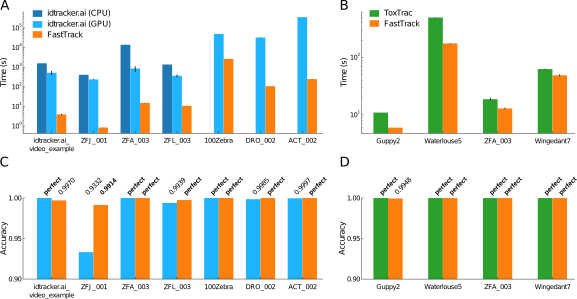
\includegraphics[width=\textwidth]{part_1/assets/Figure_benchmark.png}
    \caption{\textbf{} }
    \label{part_1:fig_benchmark}
    \end{figure}

    The accuracy was computed as follows:
    $$ A=\frac{n_{obj}n_{img} - (2N_{swap} + N_{undetected})}{n_{obj}n_{img}}$$
    with $N_{swap}$ the number of swaps, $N_{undetected}$ the number of non-detected objects, $n_{obj}$ the number of objects, and $n_{img}$ the number of images.
    For $100Zebra$, the accuracy was computed only over the 200 first images. All the results are presented in \ref{part1_fig_benchmark}. As expected, FastTrack is several orders of magnitude faster than idtracker.ai and significantly faster than ToxTrac on all tested videos. That is mainly due to the method used, idtracker.ai using deep learning and ToxTrac cost optimization and the identity preservation algorithm.
    All software performed exceptionally well in terms of accuracy, except idtracker.ai on $ZFJ\_001$ probably because the resolution is not good enough.
    FastTrack's ergonomic post-processing interface can be used to reach a perfect tracking accuracy within a few more minutes. This built-in manual correction is not possible in ToxTrac and lacking ergonomy in Idtracker.ai.

    Altogether, FastTrack offers many assets compared to idtracker.ai and ToxTrac. The software is more versatile than its concurrents and more comfortable to use. The total time spent to track a movie is globally lower, in some cases by orders of magnitude, without sacrificing tracking accuracy.

	\section{Dataset classification}
    Analyzing movies from systems as different as those compiled in $TD^2$ is a real challenge. That is partly due to the recording conditions that can be very diverse and make object detection more complex. Two recurring difficulties can be discerned: variations in illumination (e.g., reflection in GRA\_001, shadows in SOC\_001) and overlapping objects (e.g., HXB\_001).

    In movies from the academic world, systems are often designed to limit or circumvent these two difficulties. It is common to find movies with a uniform and constant illumination. Also, quasi-2D confinement and a restricted number of objects in the camera field reduce the number of occlusions.

    In $TD^2$, 23 movies have an illumination good enough to be analyzed directly with FastTrack. The others had to undergo a specific individual pre-processing before being analyzed. Two movies with too many occlusions were discarded (HXB\_001 and ZFL\_001) because they could not be analyzed with FastTrack.
    The remaining 39 films could be analyzed with FastTrack without difficulty. The Kuhn-Munkres algorithm being of complexity $O(n^3)$ the calculation time is generally quite fast. Each film was then manually corrected using the built-in tool to get the ground-truth tracking.

    FastTrack is designed to keep the post-processing phase as light as possible. However, this phase workload varies greatly depending on the movie being analyzed. This workload can be quickly estimated for a given film by computing what we call the probability of incursion.

    First, we define the incursion as the exit of an object from its Voronoi cell (\ref{} TODO RAPPEL VORONOI ANNEXE), defined at a time $t$, after a travel time $\tau$. The number of incursions depends on
    \begin{itemize}
    \item the distribution of the displacements,
    \item the density of objects,
    \item the geometry of the Voronoi cell
    \item the degree of motion alignment of the displacements.
    \end{itemize}
    To consider the objects' density, we defined the reduced length $\rho=r\sqrt{d}$ where $r$ is the length and $d$ the density. We remark that typically $\rho=1$ is corresponding to the length between two objects, and $\rho=0.5$ is the length between an object and its Voronoï cell boundary.

    Assuming that the dynamic is uncorrelated with the geometric proprieties of the Voronoï cells, we can write the incursion probability as follows:
        $$P_{inc}=\int_{0}^{\inf} R(\rho)p_{inc}(\rho) \,d \rho$$
    where $R(\rho)$ the distribution of the reduced displacement at the timescale $\rho$, and $p_{inc}(\rho)$ the geometrical probability of incursion.

    $p_{inc}(\rho)$ depends only on the geometrical properties of the objects' arrangement. We can calculate $p_{inc}$ by taking a Voronoï cell and determining the proportion of the angles for which a displacement of $\rho$ implies an incursion in a neighboring Voronoi cell. In other words, see figure~\ref{part_1:fig_pinc}, we take a circle of radius $\rho$ centered on the object and count $\Sigma$ the proportion of the circle that lies outside the Voronoï cell. That will give us $p(\rho)=\frac{\Sigma(\rho)}{2\pi}$ the geometric probability of incursion for one cell. Then, to take into account the diversity of size and shape of Voronoï cells, we average over all the cells of the movies $p_{inc}(\rho)=<p(\rho)>_{cells}$.

    Intuitively, we see that $p_{inc}$ goes from 0 when $\rho->\inf$, to 1 when $\rho>>1$. The precise shape of the geometric probability is sensitive to the density of objects, compact (e.g., ACT\_002), sparse (e.g., PAR\_001), and to the overall size of the system when walls restrict it (e.g., ZFA\_001).

	\begin{figure}[h!]
    \centering
    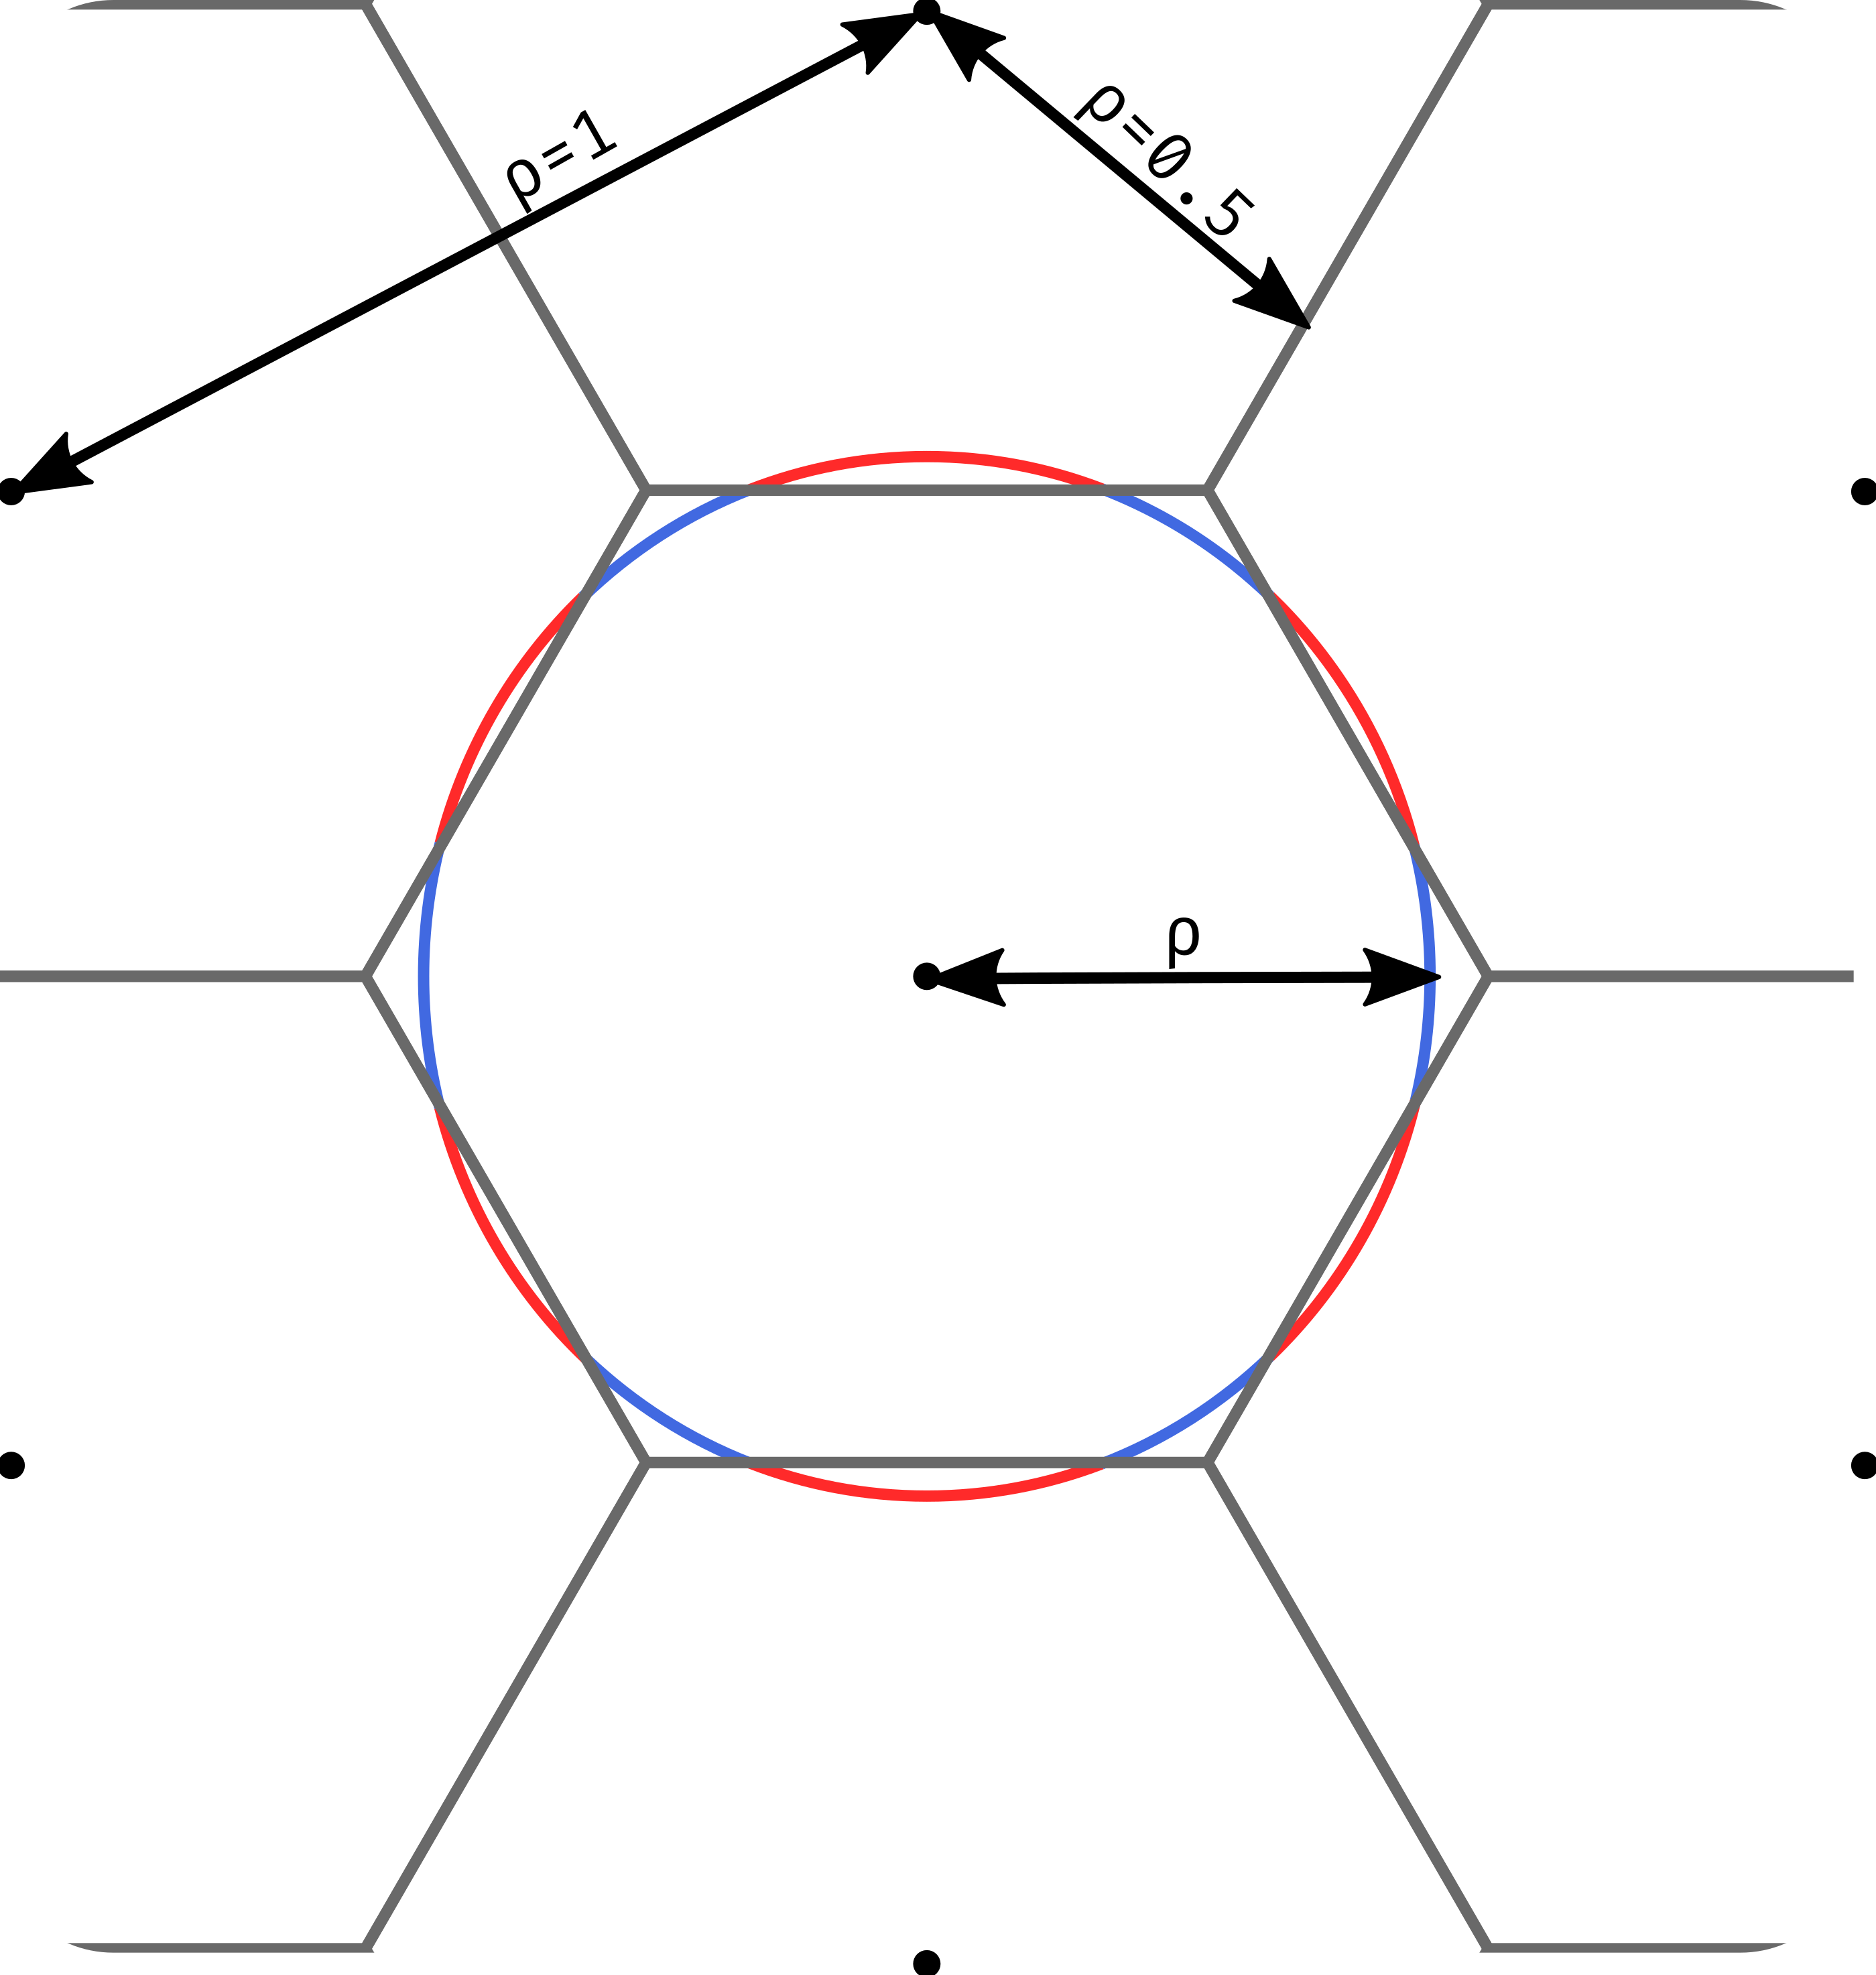
\includegraphics[width=0.5\textwidth]{part_1/assets/Figure_pinc.png}
    \caption{\textbf{Geometric probability of incursion:} Voronoï cells in black and objects black dots with typical $\rho$ length. Circle of radius $\rho$ with portions inside the Voronoï cell in blue and outside in red. The geometric probability for one cell is computed as $p(\rho)=\frac{\color{red}{\Sigma(\rho)_{out}}}{\color{red}{\Sigma(\rho)_{out}} + \color{blue}{\Sigma(\rho)_{in}}} = \frac{\color{red}{\Sigma(\rho)_{out}}}{2\pi}$}
    \label{part_1:fig_pinc}
    \end{figure}

    The distribution $R(\rho)$ is shown in \ref{part_1:fig_3}.B for three timescales $\tau$. A graphical way of calculating $P_{inc}$ is to take the intersection of the areas under $R(\rho)$ and $p_{inc}(\rho)$. In the regime where $R(\rho)$ and $p_{inc}(\rho)$ are well-separated, the resulting value of $P_{inc}$ are low but highly sensitive to the number of swaps in the tracking. Indeed, the swaps create a bump in $R$  at values of $\rho$ close to one that can artificially increase $P_{inc}$ of several orders of magnitude. Unless the ground-truth trajectories are accessible, the single value of $P_{inc}$ at $\tau=1$ can not be used as a measure for a movie's trackability.

    A timescale-varying analysis will allow us to extract more robust quantifiers. As $p_{inc}(\rho)$ does not depend on $\tau$ and $R(\rho)$ is shifted to the high values of $\rho$ when $\tau$ increases, we can expect that $P_{inc}(\tau)$ has a sigmoid-like shape. We thus computed $P_{inc}$ for various $\tau$. If $\tau>1$ we take integer values (i.e. keep one frame every $\tau1$), and if $\tau<1$ we linearly interpolated the displacements (i.e. multiplied $\rho$ by $\tau$). We represented the results in \ref{part_1:fig_3}.C for the 39 movies that could be tracked in the dataset.

    Strikingly, all $P_{inc}$ followed a logistic curve when $\tau$ is log-scaled. Therefore we used a fit of the form:
    $$Pinc=\frac{L}{1 + e^{-k(log(\tau)-x_0)}}$$
    and, noting $\tau_0=e^{x_0}$, the fitting function can be rewritten as:
    $$P_{inc}=\frac{L}{1 + \frac{\tau_0}{\tau}^k}$$
    The fits are shown in \ref{}, and are valid for all the movies in the dataset. We can make all fitting curves collapse on a single master curve. We show in \ref{part_1:fig_3}.D that $\frac{P_{inc}}{L}$ plotted as a function of $klog(frac{\tau}{\tau_0})$ follows the standard logistic sigmoid function $$f(x) =\frac{1}{1+e^{-x}}$$.

    An exciting outcome of this approach is determining the framerate at which experiments should be recorded. It is indeed a recurrent experimental question. A high temporal resolution is preferable to reduce the number of incursions and ease the tracking. However, it may not always be accessible (e.g., limited sensor rate, intense illumination required as the exposure time drops) and generates large amounts of images to store and process. A low temporal resolution can make the tracking difficult by increasing the number of incursions.
    We define $\tau_1$, the timescale at which $P_{inc}$ reaches the inverse of the total number of objects on all frames $N_{obj}$, i.e., the probability of a single incursion in the whole movie. As $\tau_1$ defines the onset of incursions and the possibility of swaps in the tracking procedure, it can be used to indicate each movie's sampling quality. Movies with $\tau_1<1$ already have incursions at the current framerate and are thus undersampled. Whereas for movies with $\tau_1>1$, the current framerate can be degraded without triggering incursions and are thus oversampled. Besides, $\tau_1$ is directly the resampling factor that one should use to have minimal movie size without generating incursions. Using \ref{}, it reads:
    $$\tau_1=\tau_0(LN_{obj}-1)^{\frac{1}{k}}$$
    We computed and ordered the values of $\tau_1$ in \ref{part_1:fig_3}.D for the whole dataset. It appears that three quarters (30) of the movies are oversampled. Any difficulty in the tracking should not be expected concerning incursions. On the other hand, nine movies are undersampled. These recordings were already known to be difficult to track, three of them ($ACT\_003$, $ACT\_004$, and $GRA\_003$) have required specific algorithms for analysis, and two ($BAC\_001$, $ZFA\_001$) required dedicated software.

    Then, we tested to what extent this characterization is robust to swaps in the trajectories. Starting from the ground truth trajectories of $ACT\_002$, we degraded the tracking quality by introducing random swaps between neighboring objects. This process is controlled by a degradation rate $\delta$, defines as the number of artificial swaps divided by the total number of objects on all frames. Such a degradation affects the small timescales more severely, and the multi-scale approach takes on its full interest. As depicted in \ref{part_1:fig_3}.F, the fits of $P_{inc}(\tau)$ are insensitive to degradation up to a remarkably high-level of $\delta \approx 10^{-3}$. Therefore, even poor-quality tracking can be used as an input for this method. As long as the distribution of displacements is only marginally affected, the output remains unchanged.

    \begin{figure}[h!]
    \centering
    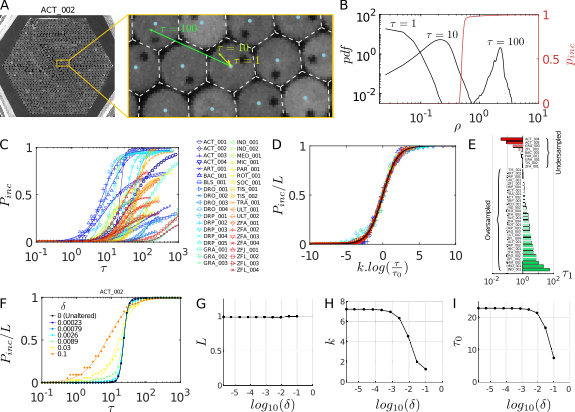
\includegraphics[width=1\textwidth]{part_1/assets/Figure_3.png}
    \caption{\textbf{}}
    \label{part_1:fig_3}
    \end{figure}

    \section{Parameters optimization}
    One may also want to determine the optimal tracking parameters, i.e., with a $P_{swap}$ close to 0 as possible. Provided that the ground-truth is known for at least one movie of a system, for example, by a careful manual post-processing. It is possible to leverage FastTrack's speed to explore the parameters space and minimize $P_{swap}$. The optimized parameters found that way can be used to track other similar movies with a minimal error rate. The workflow of the method is depicted in the Figure~\ref{part_1:fig_4}-A. As the exploration of the whole parameters space requires to perform at least thousands of trackings, such an approach is only made possible by the command-line interface (CLI) and the speed of execution of FastTrack.

    Let us first apply this approach to gain insight into the influence of $h_r$, i.e., the maximal distance allowed for an object to travel before considered lost. The Figure~\ref{part_1:fig_4}-B displays how $P_{swap}$ evolves as a function of $h_r$ for three recordings in the dataset. For low values of $h_r$, $P_{swap}$ is essentially imposed by the distribution of the objects' displacements since a high number of errors are generated when the objects are not allowed to move sufficiently. For higher values of $h_r$, the distribution of the distances to the neighbors (as defined by the Voronoï tesselation) starts to influence $P_{swap}$ as the algorithm becomes sensitive to incursions. It can also be more easily fooled by entries and exits at the boundaries of the region of interest when the number of objects in the scene varies.
    In between, for most recordings, there is a gap yielding the minimal probability of error. That is particularly true when the objects are densely packed, since the distribution of distances to neighbors is sharper, like for $DRP\_001$ where $P_{swap}$ drops to zero on a range of $h_r$. The acquisition framerate also has an essential role in this effect. With highly time-resolved movies, the distribution of displacements is shifted to the left (i.e., short distances), leading to a clear separation between the distribution of displacements and the distribution of the distances to the neighbors, resulting in low values of $P_{swap}$. In contrast, for poorly time-resolved movies like $ZFJ\_001$ the two distributions overlap, and $P_{swap}$ is always bound to high values.

    Similar analysis can be performed on the other tracking parameters. The Figure~\ref{part_1:fig_4}-C represents $P_{swap}$ as a function of both hard parameters $h_r$ and $h_t$ for $PAR\_001$, and a thin optimal segment appears. The Figure~\ref{part_1:fig_4}-D represents $P_{swap}$ as a function of the two soft parameters $s_r$ and $s_\alpha$, and an optimal ratio lies at $\frac{s_r}{s_\alpha} \simeq 0.63$. Altogether, a set of optimal parameters can be derived and used for the processing of similar recordings.

    \begin{figure}[h!]
    \centering
    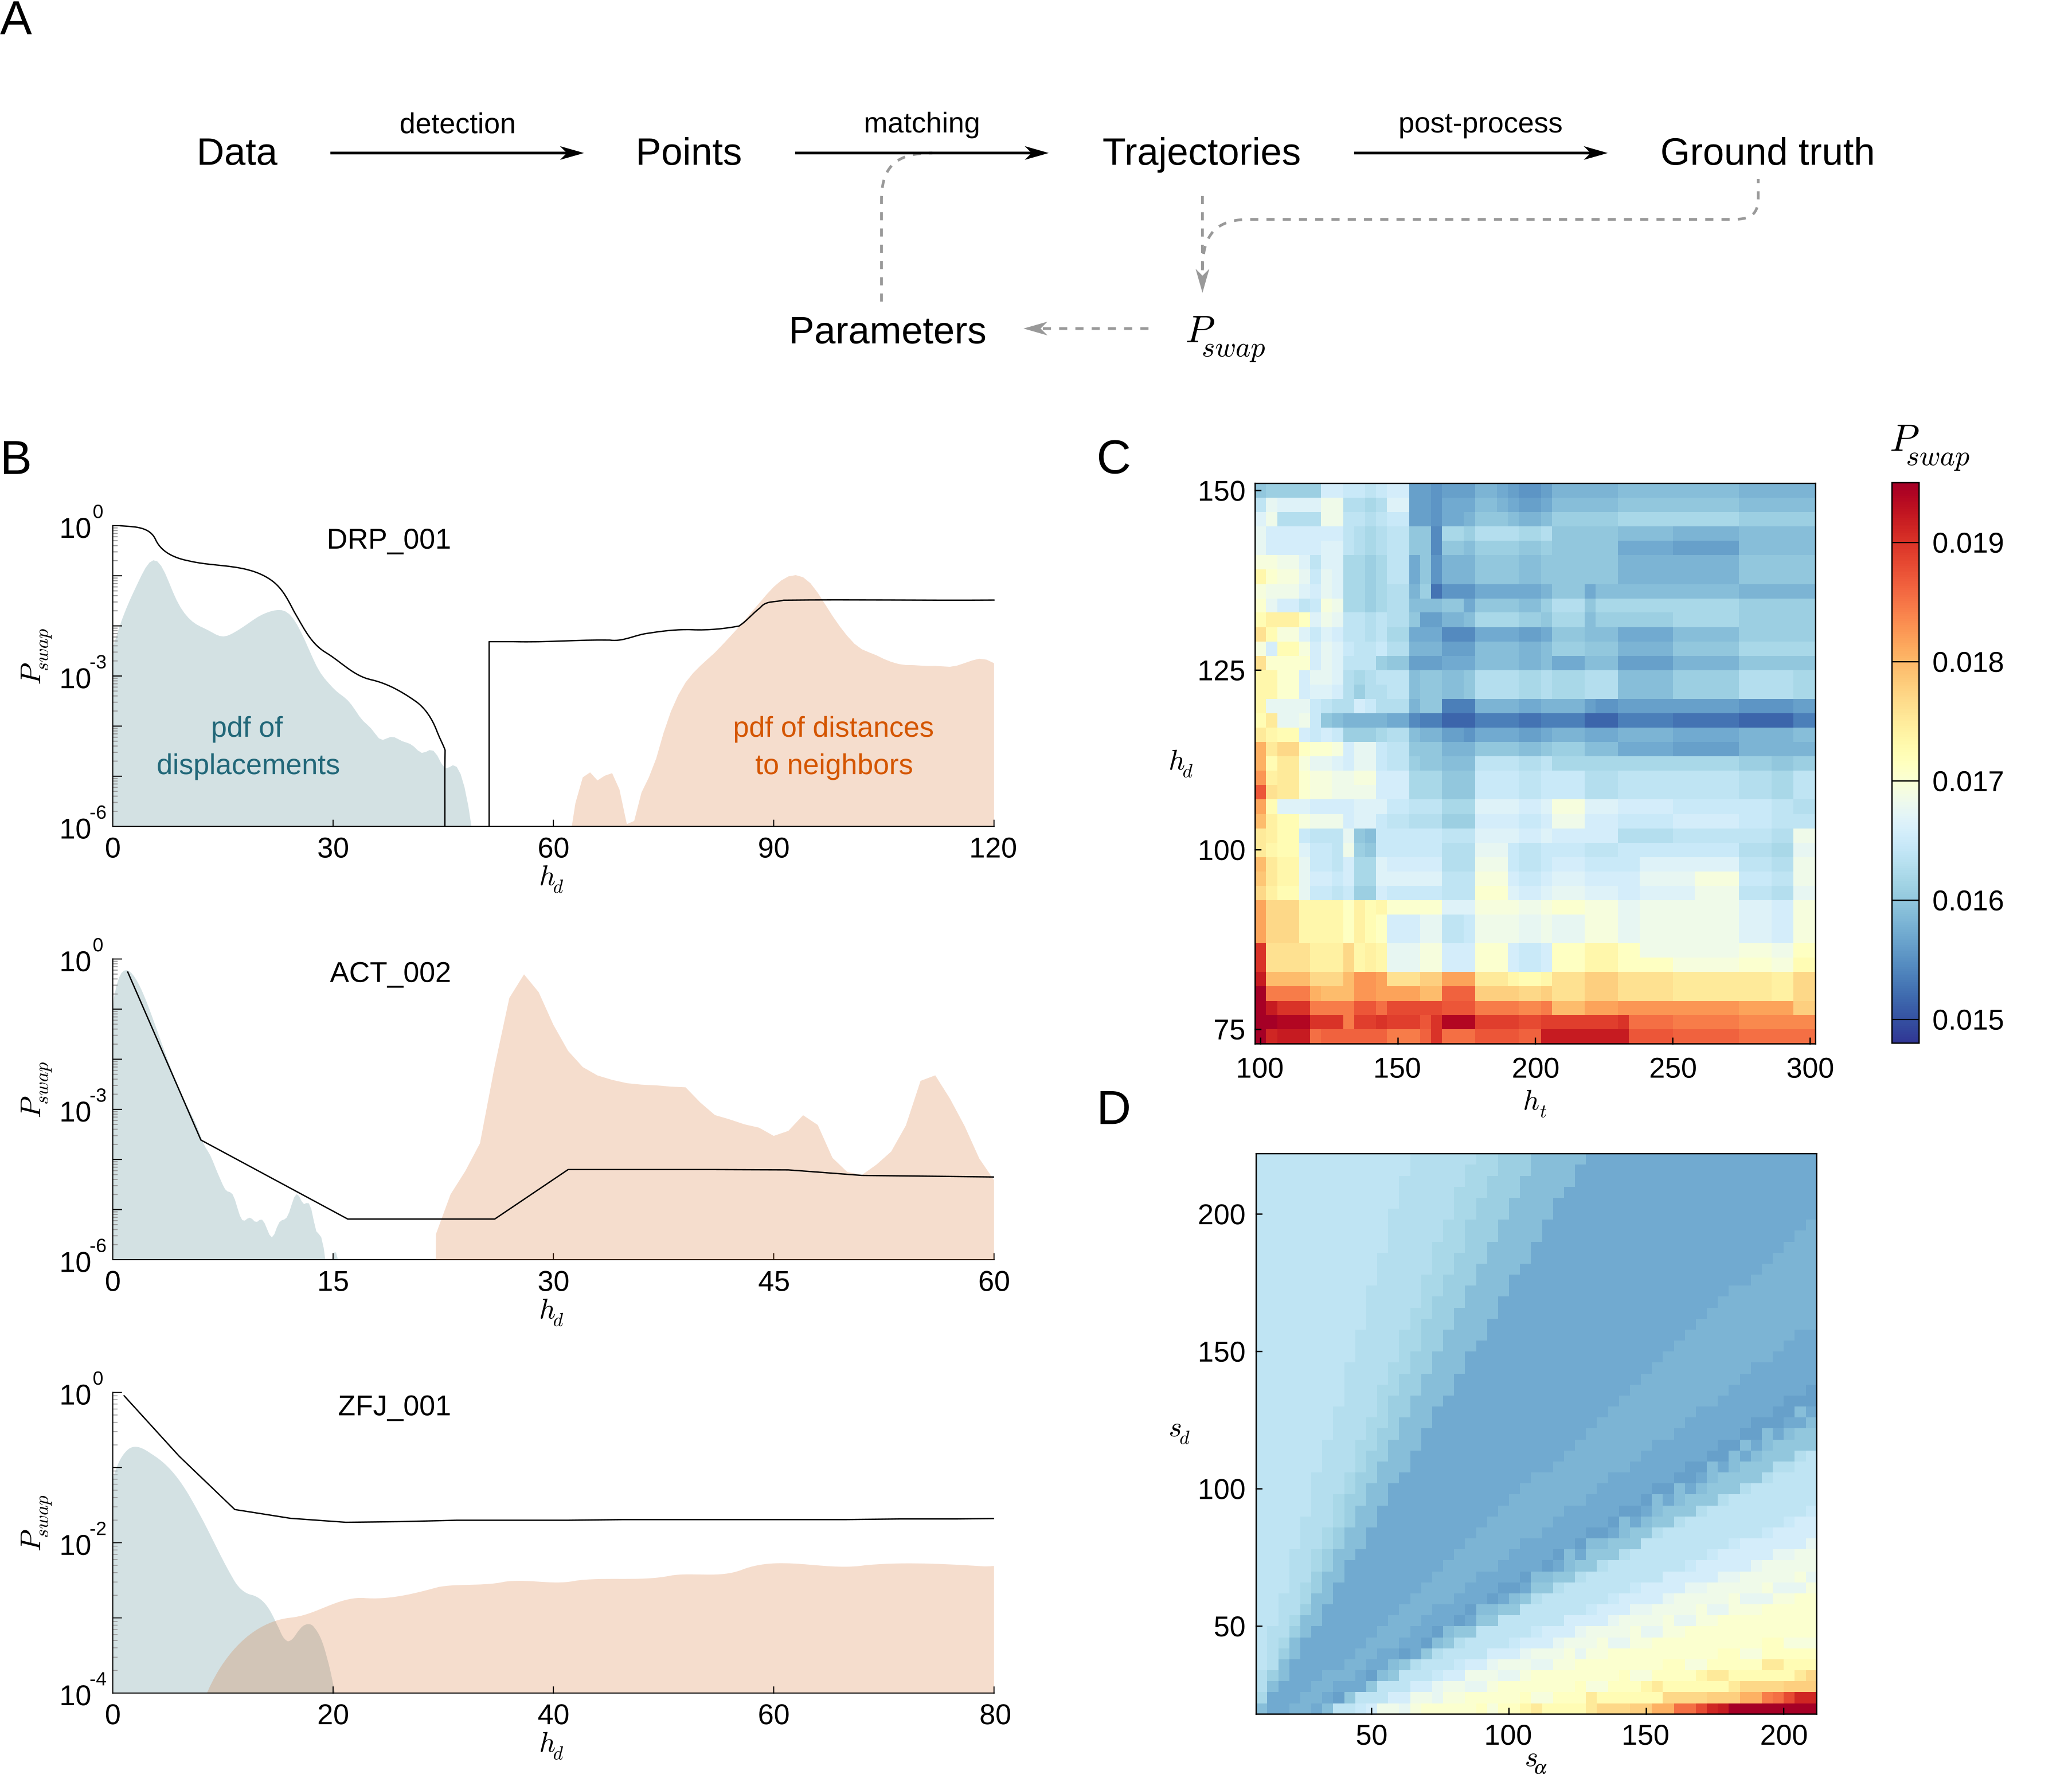
\includegraphics[width=1\textwidth]{part_1/assets/Figure_4.png}
    \caption{\textbf{}}
    \label{part_1:fig_4}
    \end{figure}
	
\chapter{Perspective}

    In this chapter, we saw how we implemented a versatile and easy to use tracking software using open-source tools. Taking advantage of the GitHub Actions system, we automated the testing and the deployment of the software, increasing confidence, and promoting collaboration. We have shown that FastTrack can compete with state-of-the-art tracking software for many usages. At the same time, we compile a database of movies to track, allowing us to benchmark tracking software on a wide variety of systems. We classify the dataset based on the probability of incursion and, doing so, highlight a criterion to determine the optimal framerate of acquisition. We have finally shown how to determine the best set of tracking parameters leveraging FastTrack capabilities.

    FastTrack's original approach, shifting the workload on the post-processing phase while keeping the pre-processing as light as possible, allows the use of FastTrack without insight into the system to track. The post-processing phase, mainly a swift checking of the tracking and small corrections, can be done directly inside the software in an interactive and ergonomic environment. FastTrack allows users to track movies quickly without any computer knowledge.

    FastTrack's approach does not prevent human inputs, mainly in the post-processing phase, to obtain a perfect tracking accuracy. It will be without inconvenience for many users who will need a human checking in any case. Users who want a perfect tracking accuracy without human input will have to turn to other tracking software that, in our knowledge, suffers severe limitations.

    It is important to note that the source code of FastTrack is available with a fully documented API. Power users can specialize the software with a custom detection phase or a custom cost function tailored to their system to circumvent any encountered limitation. The FastTrack command-line interface allows to embed the software in a high-level programming language like Python or Julia and integrate it inside an existing workflow.

    Overall, FastTrack gives any user the power to quickly analyze their movies on a relatively modest computer and power-user to build a custom-tailored software. The feedback we have encountered more frequently is how to analyze the tracking results. The standardized output leaves the user free to choose the analysis tool that he preferred. An answer to this request will be to develop analysis add-ons that can be integrated into FastTrack if needed. These add-ons will be thematic (e.g., rats behavior, soft matter), and each one will have a specific set of functions to compute meaningful quantities specific to this domain and system.
